\documentclass[a4paper,lithuanian]{article}
% Hello
\usepackage[utf8]{inputenc}
\usepackage[L7x]{fontenc}
\usepackage[lithuanian]{babel}
\usepackage{graphicx}
\usepackage{multirow}
\usepackage{amsmath}
\usepackage{amssymb}
\usepackage{multicol}
\usepackage{tikz}
\usepackage{listings}
\usepackage{color}
\usepackage{cancel}
\usepackage[normalem]{ulem}

\definecolor{dkgreen}{rgb}{0,0.6,0}
\definecolor{gray}{rgb}{0.5,0.5,0.5}
\definecolor{mauve}{rgb}{0.58,0,0.82}


\definecolor{codegreen}{rgb}{0,0.6,0}
\definecolor{codegray}{rgb}{0.5,0.5,0.5}
\definecolor{codepurple}{rgb}{0.58,0,0.82}
\definecolor{backcolour}{rgb}{0.95,0.95,0.95}


\lstdefinestyle{mystyle}{
    backgroundcolor=\color{backcolour},   
    commentstyle=\color{codegreen},
    keywordstyle=\color{blue},
    numberstyle=\color{dkgreen},
    stringstyle=\color{codepurple},
    basicstyle=\ttfamily\footnotesize,
    breakatwhitespace=false,         
    breaklines=true,                 
    captionpos=b,                    
    keepspaces=true,                 
    numbers=left,                    
    numbersep=5pt,                  
    showspaces=false,                
    showstringspaces=false,
    showtabs=false,                  
    tabsize=2
}

\lstset{style=mystyle}


\title{Algoritmų Analizė 3 N.D\\16 Variantas}

\author{
  Ričardas Čubukinas 1910620\\
  Informatika III Kursas 2 Grupė\\
  VU MIF
}

\begin{document}

\maketitle

\section{Uždavinys}
\[16.~A = [66,22,10,50,80,13,49,72]\]
\begin{lstlisting}[language=Pascal]
66 < 22 ? FALSE
10 < 50 ? TRUE
22 < 10 ? FALSE
22 < 50 ? TRUE
66 < 50 ? FALSE
80 < 13 ? FALSE
49 < 72 ? TRUE
13 < 49 ? TRUE
80 < 49 ? FALSE
80 < 72 ? FALSE
10 < 13 ? TRUE
22 < 13 ? FALSE
22 < 49 ? TRUE
50 < 49 ? FALSE
50 < 72 ? TRUE
66 < 72 ? TRUE
\end{lstlisting}
\pagebreak
\section{Uždavinys}
\[16.~40000000\]
\subsection*{(a) 16-ėje skaičiavimo sistemoje;}
$40000000 = 2500000 * 16+\mathbf{0},~2500000 = 156250 * 16+\mathbf{0},~156250 = 9765 * 16 + \mathbf{10},~9765=610 * 16 + \mathbf{5},~610=38*16+\mathbf{2},~38=2*16+\mathbf{6},~2=0*16+\mathbf{2}$
\[2625A00\]

\subsection*{(b) Mišrioje skaičiavimo sistemoje su pagrindais 60, 60, 24, 7, 52}
$40000000 = 666666 * 60 + \mathbf{40},~666666=11111 * 60 + \mathbf{6},~11111=462 * 24 + \mathbf{23},~462=66 * 7 +\mathbf{0},~66 = 1 * 52 + \mathbf{14}$\\
1 m. 14 sav. 0d. 23 val. 6 min. 40 sek.

\subsection*{(c) Liekanų vektoriumi, naudojant tarpusavyje pirminius skaičius 92, 93, 95, 97}

\[40000000 \mod 92 = 56\]
\[40000000 \mod 93 = 49\]
\[40000000 \mod 95 = 60\]
\[40000000 \mod 97 = 13\]
\[(56,49,60,13)\]
\pagebreak
\section{Uždavinys}
\[16.~E = \{(A, E), (B, C), (A, D), (B, F), (D, B)\}\]
\subsection*{(a) Grafiškai}
\begin{center}
\begin{tikzpicture}
\node {A}
   child {
      node {D}
      child {
        node {B}
        child{
          node {C}
        }
        child{
          node {F}
        }
      }
    }
    child { node {E}};
\end{tikzpicture}
\end{center}
\subsection*{(b) Tėvų nuorodos}
\begin{center}
\begin{tabular}{c c c}
  \hline
  Indeksas & INFO & Tėvas\\
  \hline
  1 & A & NIL\\
  2 & D & 1\\
  3 & E & 1\\
  4 & B & 2\\
  5 & C & 4\\
  6 & F & 4\\
  \hline
\end{tabular}
\end{center}
\subsection*{(c) Vaikų nuorodos}

\begin{center}
\begin{tabular}{c c c c}
  \hline
  Indeksas & INFO & 1 vaikas & 2 vaikas\\
  \hline
  1 & A & 2 & 3\\
  2 & D & 4 & NIL\\
  3 & E & NIL & NIL\\
  4 & B & 5 & 6\\
  5 & C & NIL & NIL\\
  6 & F & NIL & NIL\\
  \hline
\end{tabular}
\end{center}

\subsection*{(d) Nurodant kairyjį vaiką ir dešinyjį brolį}
\begin{center}
\begin{tabular}{c c c c}
  \hline
  Indeksas & INFO & Kairysis vaikas & Dešinysis brolis\\
  \hline
  1 & A & 2 & NIL\\
  2 & D & 4 & 3\\
  3 & E & NIL & NIL\\
  4 & B & 5 & NIL\\
  5 & C & NIL & 6\\
  6 & F & NIL & NIL\\
  \hline
\end{tabular}
\end{center}
\pagebreak
\section{Uždavinys}
\[16.~\vec{b}=(4, 1, 2, 1, 3, 3, 4, 2, 4, 1, 4) \]
\subsection*{(a) Grafiškai}
\begin{center}
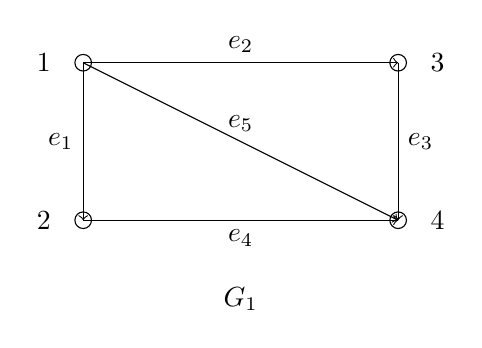
\begin{tikzpicture}
        \draw[] (0,0) circle (3pt);
        \draw[] (4,0) circle (3pt);
        \draw[] (4,2) circle (3pt);
        \draw[] (0,2) circle (3pt);
        
        % labelleds
        \node at (-0.5,2) {$1$};
        \node at (-0.5,0) {$2$};
        \node at (4.5,2) {$3$};
        \node at (4.5,0) {$4$};
        \node at (2,-1) {$G_1$};
        %% arcs
        \draw[->] (0,2) -- node [left] {$e_1$} (0,0);
        \draw[->] (0,2) -- node [above] {$e_2$} (4,2);
        \draw[->] (4,2) -- node [right] {$e_3$} (4,0);
        \draw[->] (0,0) -- node [below] {$e_4$} (4,0);
        \draw[->] (0,2) -- node [above] {$e_5$} (4,0);
\end{tikzpicture}
\end{center}
\subsection*{(b) Gretimumo (jungumo) matrica}
\begin{center}
$A_1=$
\begin{pmatrix}
  0 & 1 & 1 & 1\\
  1 & 0 & 0 & 1\\
  1 & 0 & 0 & 1\\
  1 & 1 & 1 & 0
\end{pmatrix}
\end{center}

\subsection*{(c) Gretimumo struktūra}
\[1\rightarrow{}2\rightarrow{}3\rightarrow{}4\rightarrow{}\text{nil}\]
\[2\rightarrow{}1\rightarrow{}4\rightarrow{}\text{nil}\]
\[3\rightarrow{}1\rightarrow{}4\rightarrow{}\text{nil}\]
\[4\rightarrow{}3\rightarrow{}2\rightarrow{}1\rightarrow{}\text{nil}\]
\subsection*{(d) Incidencijų matrica}
\begin{center}
$B_1=$
\begin{pmatrix}
  1 & 1 & 0 & 0 & 1\\
  1 & 0 & 0 & 1 & 0\\
  0 & 1 & 1 & 0 & 0\\
  0 & 0 & 1 & 1 & 1\\
\end{pmatrix}
\end{center}

\end{document}
